\documentclass[conference]{IEEEtran}
\usepackage[utf8]{inputenc}
\usepackage[T1,T5]{fontenc}
\usepackage{textcomp}
\usepackage{listings}
\usepackage{graphicx}
\usepackage{booktabs}
\usepackage{hyperref}
\usepackage{cite}
\usepackage{amsmath}
\begin{document}
\title{Evaluating Qwen2.5-7B Few-shot Prompting Against GPT-4o Threshold for Bug Report Quality Assessment}
\author{
\IEEEauthorblockN{Phan Hoàng Thông, Huỳnh Kha Thanh Hoàng, Nguyễn Công Huy, Lại Minh Dũng, Võ Thanh Phong}
\IEEEauthorblockA{FPT University, Vietnam \\
\{SE194047, SE193944, SE192333, SE194215, SE194101\}@fpt.edu.vn}
}
\maketitle
\begin{abstract}
Bug reports provide the information developers need to triage and resolve software defects, yet unclear or unstructured reports delay this process. Existing work on Qwen2.5-7B consistently relies on supervised fine-tuning or reinforcement learning before evaluation, while GPT-4o serves only as a few-shot baseline; no study has examined whether Qwen2.5-7B under few-shot prompting only -- without additional training -- can match the GPT-4o thresholds established by Acharya and Ginde (2025) (CTQRS $\geq$75\%, ROUGE-1 $\geq$0.47, SBERT $\geq$0.82). We evaluate Qwen2.5-7B-Instruct with 3-shot prompting on 262 Bugzilla bug reports, measuring CTQRS, ROUGE-1 F1, and SBERT cosine similarity against these thresholds using one-sample Wilcoxon signed-rank tests. Qwen2.5-7B exceeds the CTQRS threshold (median=88.89\%, $p<0.001$, Cliff's $\delta$=0.908) and the ROUGE-1 threshold (median=0.491, $p$=0.002, $\delta$=0.191), but falls short of the SBERT threshold (median=0.632, $p$=1.000, $\delta$=-0.969); a length-constrained ablation raises ROUGE-1 to 0.532 but SBERT remains at 0.609, indicating stylistic verbosity rather than semantic inaccuracy. These results show that few-shot prompting alone lets an open-source LLM match GPT-4o's structural and lexical quality without additional training, but output style remains the key barrier to semantic-similarity metrics.
\end{abstract}
\begin{IEEEkeywords}
large language models, bug report quality, few-shot prompting, CTQRS, empirical study
\end{IEEEkeywords}
\section{Introduction}
\label{sec:intro}

Bug reports are the primary communication channel between end users and 
development teams in software maintenance, providing developers with 
critical information to identify, triage, and resolve software defects~\cite{acharya2025bugquality}. 
However, the effectiveness of bug reports is often hindered by ambiguity, 
incompleteness, or inconsistency in the information provided by 
reporters~\cite{acharya2025bugquality}. Well-structured reports that clearly articulate 
Steps to Reproduce (S2R), Expected Behavior (EB), and Actual Behavior (AB) 
minimize ambiguity and enable developers to resolve issues without extensive 
discussion and clarification~\cite{acharya2025bugquality}. Challenges in bug reporting 
persist due to factors such as varying reporter experience and difficulty in 
providing essential details like reproduction steps and expected 
outcomes~\cite{acharya2025bugquality}.

Recent advances in large language models (LLMs) have opened a promising 
direction: automatically restructuring unstructured bug descriptions into 
well-formed reports. Proprietary models such as GPT-4o have demonstrated 
strong few-shot performance on this task, achieving CTQRS=75\% and 
SBERT=0.82 in 3-shot setting~\cite{acharya2025bugquality}. Open-source 
alternatives such as Qwen2.5-7B have shown competitive results when 
fine-tuned on domain-specific datasets, reaching CTQRS=77\% after 
instruction fine-tuning~\cite{acharya2025bugquality}, CTQRS=80.5\% with 
QLoRA-4bit multi-agent pipeline~\cite{choi2025agentreport}, and 
CTQRS=0.76 with PPO reinforcement learning~\cite{yang2025ctqrsrl}. 
The Crowdsourced Test Report Quality Score (CTQRS)~\cite{zhang2022ctqrs} 
has emerged as a principled metric for evaluating structural completeness 
of generated reports, complementing lexical (ROUGE-1) and semantic (SBERT) 
similarity measures.

However, a critical gap remains in the literature. Existing work on 
Qwen2.5-7B consistently relies on supervised fine-tuning (LoRA, QLoRA) or 
reinforcement learning before evaluation~\cite{acharya2025bugquality, choi2025agentreport, yang2025ctqrsrl}. 
No prior study has examined whether Qwen2.5-7B under \emph{few-shot prompting only} 
--- without any additional training --- can match the quality thresholds 
achieved by GPT-4o in the same few-shot setting. This distinction matters 
practically: organizations with constrained GPU budgets may prefer a 
zero-training-cost deployment, yet without empirical evidence, they cannot 
make an informed choice between few-shot prompting and investing in fine-tuning.

In this paper, we address this gap with a controlled empirical study. 
We apply Qwen2.5-7B-Instruct with 3-shot prompting (Alpaca-LoRA template, 
following~\cite{acharya2025bugquality}) to 262 Bugzilla bug reports from 
the GindeLab dataset~\cite{acharya2025bugquality} and measure CTQRS, 
ROUGE-1 F1, and SBERT cosine similarity against the thresholds published 
for GPT-4o 3-shot. Statistical significance is assessed using the 
Wilcoxon signed-rank one-sample test ($\alpha = 0.05$) with Cliff's $\delta$ 
as the effect size measure~\cite{arcuri2011practical}. 
To our knowledge, this is the first study to directly evaluate 
Qwen2.5-7B few-shot performance against established GPT-4o few-shot 
thresholds on the bug report restructuring task.

To summarize, this paper contributes:
\begin{enumerate}
    \item The first empirical evaluation of Qwen2.5-7B-Instruct 3-shot 
    prompting for bug report quality assessment using CTQRS, ROUGE-1, 
    and SBERT on the Bugzilla dataset (N=262).
    
    \item Experimental results showing mixed outcomes: Qwen2.5-7B 
    few-shot achieves CTQRS=88.89\% (p$<$0.001, $\delta$=0.908) and 
    ROUGE-1=0.491 (p=0.002, $\delta$=0.191) above the GPT-4o thresholds, 
    but SBERT=0.632 (p=1.000, $\delta$=-0.969) below threshold --- 
    attributable to output style mismatch rather than semantic content errors.
    
    \item An ablation study demonstrating that length-constraining the 
    prompt improves ROUGE-1 (0.491$\rightarrow$0.532) but does not resolve 
    the SBERT gap (0.632$\rightarrow$0.609), providing evidence that 
    fine-tuning remains necessary for style alignment.
    
    \item A public replication package including dataset, prompts, scripts, 
    and raw results available at: 
    \url{https://github.com/HoangThong05/RT-SWT-003-nhom3}.
\end{enumerate}

The remainder of this paper is structured as follows. 
Section~\ref{sec:related} reviews related work. 
Section~\ref{sec:method} describes the experimental methodology. 
Section~\ref{sec:results} presents results. 
Section~\ref{sec:discussion} discusses findings and implications. 
Section~\ref{sec:threats} addresses threats to validity. 
Section~\ref{sec:conclusion} concludes.


\section{Related Work}
\label{sec:related}

\subsection{Bug Report Quality Assessment and Generation}

Early work on bug report quality used heuristic rules and
machine learning to detect incomplete or ambiguous reports.
Chaparro et al. assessed the quality of Steps to Reproduce
(S2R) using grammar parsing and neural sequence
labelling~\cite{chaparro2019assessing}. Zhang et al.
proposed CTQRS~\cite{zhang2022ctqrs}, a rule-based framework
that scores reports across morphological, relational, and
analytical dimensions. These studies established the
evaluation criteria that later LLM-based approaches inherited.

More recent work has shifted from detecting quality issues to
automatically fixing them using LLMs. Bo et al.~\cite{bo2024chatbr}
(ChatBR) combined a BERT-based detector with GPT-3.5-turbo to
generate missing information, achieving precision improvements
of 25.38--29.20\% over prior methods on six OSS projects.
Akyol et al.~\cite{akyol2026improbr} (ImproBR) used a
retrieval-augmented pipeline with GPT-4o mini to improve
Mojira/Minecraft reports, increasing the proportion of
complete reports from 7.9\% to 96.4\%. These approaches
demonstrate the effectiveness of proprietary LLMs in
few-shot or RAG settings, but rely on commercial APIs
that impose cost and privacy constraints.

\subsection{Open-Source LLMs with Training Adaptation}

To address cost and privacy limitations of proprietary
models, several studies have fine-tuned open-source LLMs
for bug report generation.
Acharya and Ginde~\cite{acharya2025bugquality} instruction
fine-tuned Qwen2.5-7B, Mistral-7B, and Llama3.2-3B on the
Bugzilla dataset (N=3,903) using the Alpaca-LoRA template,
with GPT-4o 3-shot as the reference baseline. Their
fine-tuned Qwen2.5-7B achieved CTQRS=77\%, ROUGE-1=0.61,
SBERT=0.85 versus GPT-4o 3-shot at CTQRS=75\%,
ROUGE-1=0.47, SBERT=0.82.
Choi and Yang~\cite{choi2025agentreport} (AgentReport)
applied QLoRA-4bit with a multi-agent pipeline on the same
Bugzilla corpus, reaching CTQRS=80.5\%.
Yang~\cite{yang2025ctqrsrl} further trained Qwen2.5-7B with
PPO reinforcement learning using CTQRS as the reward signal,
improving CTQRS from 0.46 to 0.76.

A consistent finding across these studies is that training
adaptation --- whether supervised fine-tuning or reinforcement
learning --- is necessary to achieve competitive SBERT scores,
as untrained models produce outputs with different stylistic
characteristics than the Bugzilla reference corpus.
Dın\c{c} et al.~\cite{dinc2025quality} corroborate this:
on a 10,000-report Mozilla Firefox corpus, a fine-tuned
RoBERTa model (F1=0.909) outperformed zero-shot and
few-shot LLM approaches, highlighting the value of
domain-specific training.

\subsection{Gap and Positioning}

Across all 13 papers we reviewed, Qwen2.5-7B appears
exclusively in fine-tuned or RL-adapted
configurations~\cite{acharya2025bugquality,
choi2025agentreport, yang2025ctqrsrl}. GPT-4o and
GPT-4o mini serve as few-shot baselines in several
studies~\cite{acharya2025bugquality, akyol2026improbr},
but no study has directly evaluated whether
\emph{Qwen2.5-7B in a few-shot-only setting} can
match the quality thresholds that GPT-4o achieves
under the same prompting conditions. This gap motivates
our study: if Qwen2.5-7B few-shot can replicate
GPT-4o's few-shot performance, organizations could
deploy a capable open-source model without any training
investment.

% sections/03_method.tex
% §3 Methodology
% §3.1 + §3.2: LR — Nguyễn Công Huy (SE192333)
% §3.3 + §3.4: MS — Lại Minh Dũng (SE194215)
% Nguồn: proposal.md §5.1–§5.5, notes.md, cost_log_LR.md, compute_metrics_MS.py

\section{Methodology}
\label{sec:method}

\subsection{Dataset}
\label{sec:dataset}

We use the Bugzilla bug report dataset released by Acharya and
Ginde~\cite{acharya2025bugquality}, available at
\url{https://github.com/GindeLab/Ease_2025_AI_model}. The
dataset contains structured bug reports mined from the Mozilla
Bugzilla tracker. The raw file
(\texttt{Plus14\_filtered\_bug\_report\_scores\_Summary.xlsx})
comprises 3,966 rows and 32 columns after the authors' initial
quality filtering (requiring S2R, EB, AB, and Additional
Information, and excluding reports containing stack traces or
code snippets).

Each row pairs an \emph{unstructured input} (column
\texttt{NEW\_llama\_output}: a summary generated by Llama3
from the original report) with a \emph{structured ground truth}
(column \texttt{text}: the original Bugzilla report conforming
to the four-section template). No manual annotation was
performed; ground truth is sourced directly from Bugzilla
reporter submissions.

We split the 3,966 rows 80/10/10 (train / validation / test)
using \texttt{random\_state=42}, yielding a test set of 262
samples used for RQ1. The training partition was not used as
we evaluate few-shot prompting only.

\subsection{Experimental Setup}
\label{sec:setup}

\textbf{Model and environment.}
We use \texttt{unsloth/Qwen2.5-7B-Instruct} loaded from
HuggingFace with \texttt{torch\_dtype=float16} and
\texttt{device\_map=``auto''}. Inference runs on a Kaggle
Notebook with a Tesla T4 GPU (free tier, \$0 cost). An
initial attempt with a P100 GPU encountered a CUDA capability
incompatibility (\texttt{sm\_60} not supported); we switched
to T4 before the pilot run.

\textbf{Inference configuration.}
We set \texttt{temperature=0.01} (the minimum permitted value;
Qwen2.5-7B-Instruct requires \texttt{temperature~>~0}),
\texttt{do\_sample=False} (greedy decoding), and
\texttt{max\_new\_tokens=512}.

\textbf{Prompt design.}
We follow the Alpaca-LoRA 3-shot template from
E02~\cite{acharya2025bugquality} (Listing~2), providing
three input--output exemplar pairs drawn from the training
set before the target input. The system prompt instructs
the model to produce four sections: Steps to Reproduce
(S2R), Expected Result (ER), Actual Result (AR), and
Additional Information.

Listing~\ref{lst:prompt} shows the exact template, following
the Alpaca-style format used by E02~\cite{acharya2025bugquality}
(their Listing 2).

\begin{lstlisting}[caption={Alpaca-style prompt template used for 3-shot inference, following E02~\protect\cite{acharya2025bugquality}.}, label={lst:prompt}, basicstyle=\ttfamily\scriptsize, breaklines=true]
You are a senior software engineer specialized in
generating detailed bug reports.

### Instruction:
Please create a bug report that includes the
following sections:
1. Steps to Reproduce (S2R): Detailed steps to
   replicate the issue.
2. Expected Result (ER): What you expected to happen.
3. Actual Result (AR): What actually happened.
4. Additional Information: Include relevant details
   such as software version, build number,
   environment, etc.
If any of these sections are missing from the
provided report, explicitly notify the user which
information is missing.

### Input:
{unstructured_report}

### Response:
{Bug_report}
\end{lstlisting}

The three exemplar pairs (not shown due to space) are
sampled from the training partition; the exact instances
used are available in our replication package.

\textbf{Pilot and full run.}
We first ran a pilot on 80 samples; all 80 outputs contained
the four required sections (100\% valid), confirming pipeline
correctness. We then ran inference on all 262 test samples in
a single Kaggle session with automatic checkpointing every
20 samples. Total runtime was approximately 2.6 hours
($\approx$35 seconds per sample). All 262 outputs were
non-empty and well-formed; 0 samples were excluded. The
replication package includes all outputs in
\texttt{results/full\_llm\_output.csv} and the API log in
\texttt{results/full\_api\_log.txt}.

Our replication package, including datasets, prompts,
scripts, and raw results, is publicly available at:
\url{https://github.com/HoangThong05/RT-SWT-003-nhom3}.

\subsection{Evaluation Metrics}
\label{sec:metrics}

We evaluate generated bug reports using three complementary
metrics, following~\cite{acharya2025bugquality}.

\textbf{CTQRS (Crowdsourced Test Report Quality Score).}
CTQRS~\cite{zhang2022ctqrs} assesses structural completeness
through 13 rule-based sub-checks organized into three
categories: morphological (RM1--4), relational (RR1--5),
and analytical (RA1--4). The maximum possible score is 18
points (RM1--4: $4\times1$; RR1, RR2, RR4, RR5: $4\times1$;
RR3: $1\times2$; RA1--4: $4\times2$). We report
$\text{CTQRS\%} = (\text{raw score} / 18) \times 100$.

We identified and corrected two technical issues in the
GindeLab scorer prior to evaluation: (i) word-list noise in
RA sub-checks causing false positives, and (ii) a hardcoded
\texttt{max\_possible=16} contradicting the actual weighted
sum of 18 derivable from the scorer source code (details in
Section~\ref{sec:threats}). The corrected scorer is
available as \texttt{scripts/ctqrs\_scorer\_v2\_fixed.py}.

\textbf{ROUGE-1 F1.}
ROUGE-1~\cite{lin2004rouge} measures unigram overlap between
generated output and ground-truth reference. We use the
\texttt{rouge-score} library (v0.4.x), reporting F1 score.

\textbf{SBERT Cosine Similarity.}
We compute sentence embedding similarity using
\texttt{sentence-transformers} with model
\texttt{paraphrase-MiniLM-L6-v2}~\cite{acharya2025bugquality},
computing cosine similarity between the generated output and
the ground-truth reference embeddings.

\subsection{Statistical Analysis Plan}
\label{sec:stats}

\textbf{Test selection.}
We use the Wilcoxon signed-rank one-sample
test~\cite{arcuri2011practical} for each of the three
hypotheses in RQ1. This non-parametric test is appropriate
because the metric distributions are not guaranteed to be
normal, and we compare a sample median against a fixed
published threshold. The significance level is $\alpha = 0.05$.

\textbf{Hypotheses.}
For each metric $m \in \{\text{CTQRS}, \text{SBERT},
\text{ROUGE-1}\}$ with threshold $\tau_m$:
$H_0^m$: median$(m) < \tau_m$;
$H_1^m$: median$(m) \geq \tau_m$.
We reject $H_0^m$ when $p < 0.05$ and median$(m) \geq \tau_m$.
Thresholds are taken from Figure~4 of~\cite{acharya2025bugquality}
(GPT-4o 3-shot): CTQRS $\geq 75\%$, SBERT $\geq 0.82$,
ROUGE-1 $\geq 0.47$.

\textbf{Effect size and multiple testing.}
We report Cliff's $\delta$~\cite{arcuri2011practical}
alongside every $p$-value ($|\delta|<0.147$ negligible,
$<0.33$ small, $<0.474$ medium, otherwise large). We apply
Bonferroni correction ($\alpha_{\text{adj}} = 0.05/3
\approx 0.017$) and verify conclusions are unchanged.
% sections/04_results.tex
% §4 Results — MS (Lại Minh Dũng, SE194215)

\section{Results}
\label{sec:results}

\subsection*{RQ1: Does Qwen2.5-7B 3-shot reach the GPT-4o reference thresholds?}

The evaluation includes 262 bug reports from the Bugzilla test
set. Table~\ref{tab:results} presents the descriptive
statistics together with the outcomes of the Wilcoxon
signed-rank tests. Figure~\ref{fig:boxplot} illustrates the
distribution of the three evaluation metrics relative to the
corresponding GPT-4o reference thresholds.

\begin{table}[t]
\centering
\caption{Evaluation results of Qwen2.5-7B with 3-shot prompting
on the Bugzilla test set (N=262). The benchmark thresholds are
taken from the GPT-4o 3-shot results reported by
\protect\cite{acharya2025bugquality}.}
\label{tab:results}
\begin{tabular}{lcccccc}
\toprule
\textbf{Metric} &
\textbf{Threshold} &
\textbf{Median} &
\textbf{IQR} &
\textbf{\textit{p}-value} &
\textbf{Cliff's $\delta$} &
\textbf{Decision} \\
\midrule
CTQRS (\%) &
$\geq$75.0 &
88.89 &
[83.33, 94.44] &
$<$0.001 &
0.908 (large) &
Reject $H_0$ \\

ROUGE-1 F1 &
$\geq$0.47 &
0.491 &
[0.420, 0.551] &
0.002 &
0.191 (small) &
Reject $H_0$ \\

SBERT &
$\geq$0.82 &
0.632 &
[0.549, 0.701] &
1.000 &
$-$0.969 (large) &
Fail to reject $H_0$ \\
\bottomrule
\end{tabular}
\end{table}

\textbf{H1.1 -- CTQRS.}

CTQRS values were generally high across the evaluation set.
The median reached 88.89\%, and half of the reports obtained
scores within the interval of 83.33\% to 94.44\%. The reported
median was above the reference value of 75\%.

Statistical analysis using the Wilcoxon signed-rank test
returned $p<0.001$. The corresponding Cliff's $\delta$
was 0.908, representing a large effect size.
Accordingly, $H_0^{\text{CTQRS}}$ was rejected.

Most reports received relatively high CTQRS scores.
Specifically, 89 reports obtained 16 points, 55 obtained
17 points, and another 13 reached the maximum score of
18 points. Only 12 reports (4.6\%) scored below the
reference threshold.

\textbf{H1.2 -- SBERT.}

The SBERT similarity scores are centered around a median of
0.632. The interquartile range extends from 0.549 to 0.701,
which remains below the benchmark value of 0.82.

The statistical comparison resulted in a $p$-value of 1.000,
with Cliff's $\delta$ equal to $-0.969$, indicating a large
effect in the opposite direction. Accordingly,
$H_0^{\text{SBERT}}$ was not rejected.

\textbf{H1.3 -- ROUGE-1.}

ROUGE-1 F1 achieved a median score of 0.491.
The middle half of the observations ranged from
0.420 to 0.551, placing the median above the
reference threshold of 0.47.

The Wilcoxon signed-rank test returned
$p=0.002$, while Cliff's $\delta$ was 0.191,
representing a small effect size.
Therefore, $H_0^{\text{ROUGE-1}}$ was rejected.

\textbf{Bonferroni correction.}

To account for the three hypothesis tests performed for RQ1,
a Bonferroni correction was applied, resulting in an adjusted
significance level of
$\alpha_{\text{adj}}=0.05/3\approx0.017$.The conclusions were unchanged after applying the correction.
CTQRS ($p_{\text{adj}}<0.001$) and ROUGE-1
($p_{\text{adj}}=0.005$) continued to reject the null
hypothesis, whereas SBERT
($p_{\text{adj}}=1.000$) continued to fail to reject it.

\begin{figure}[t]
\centering
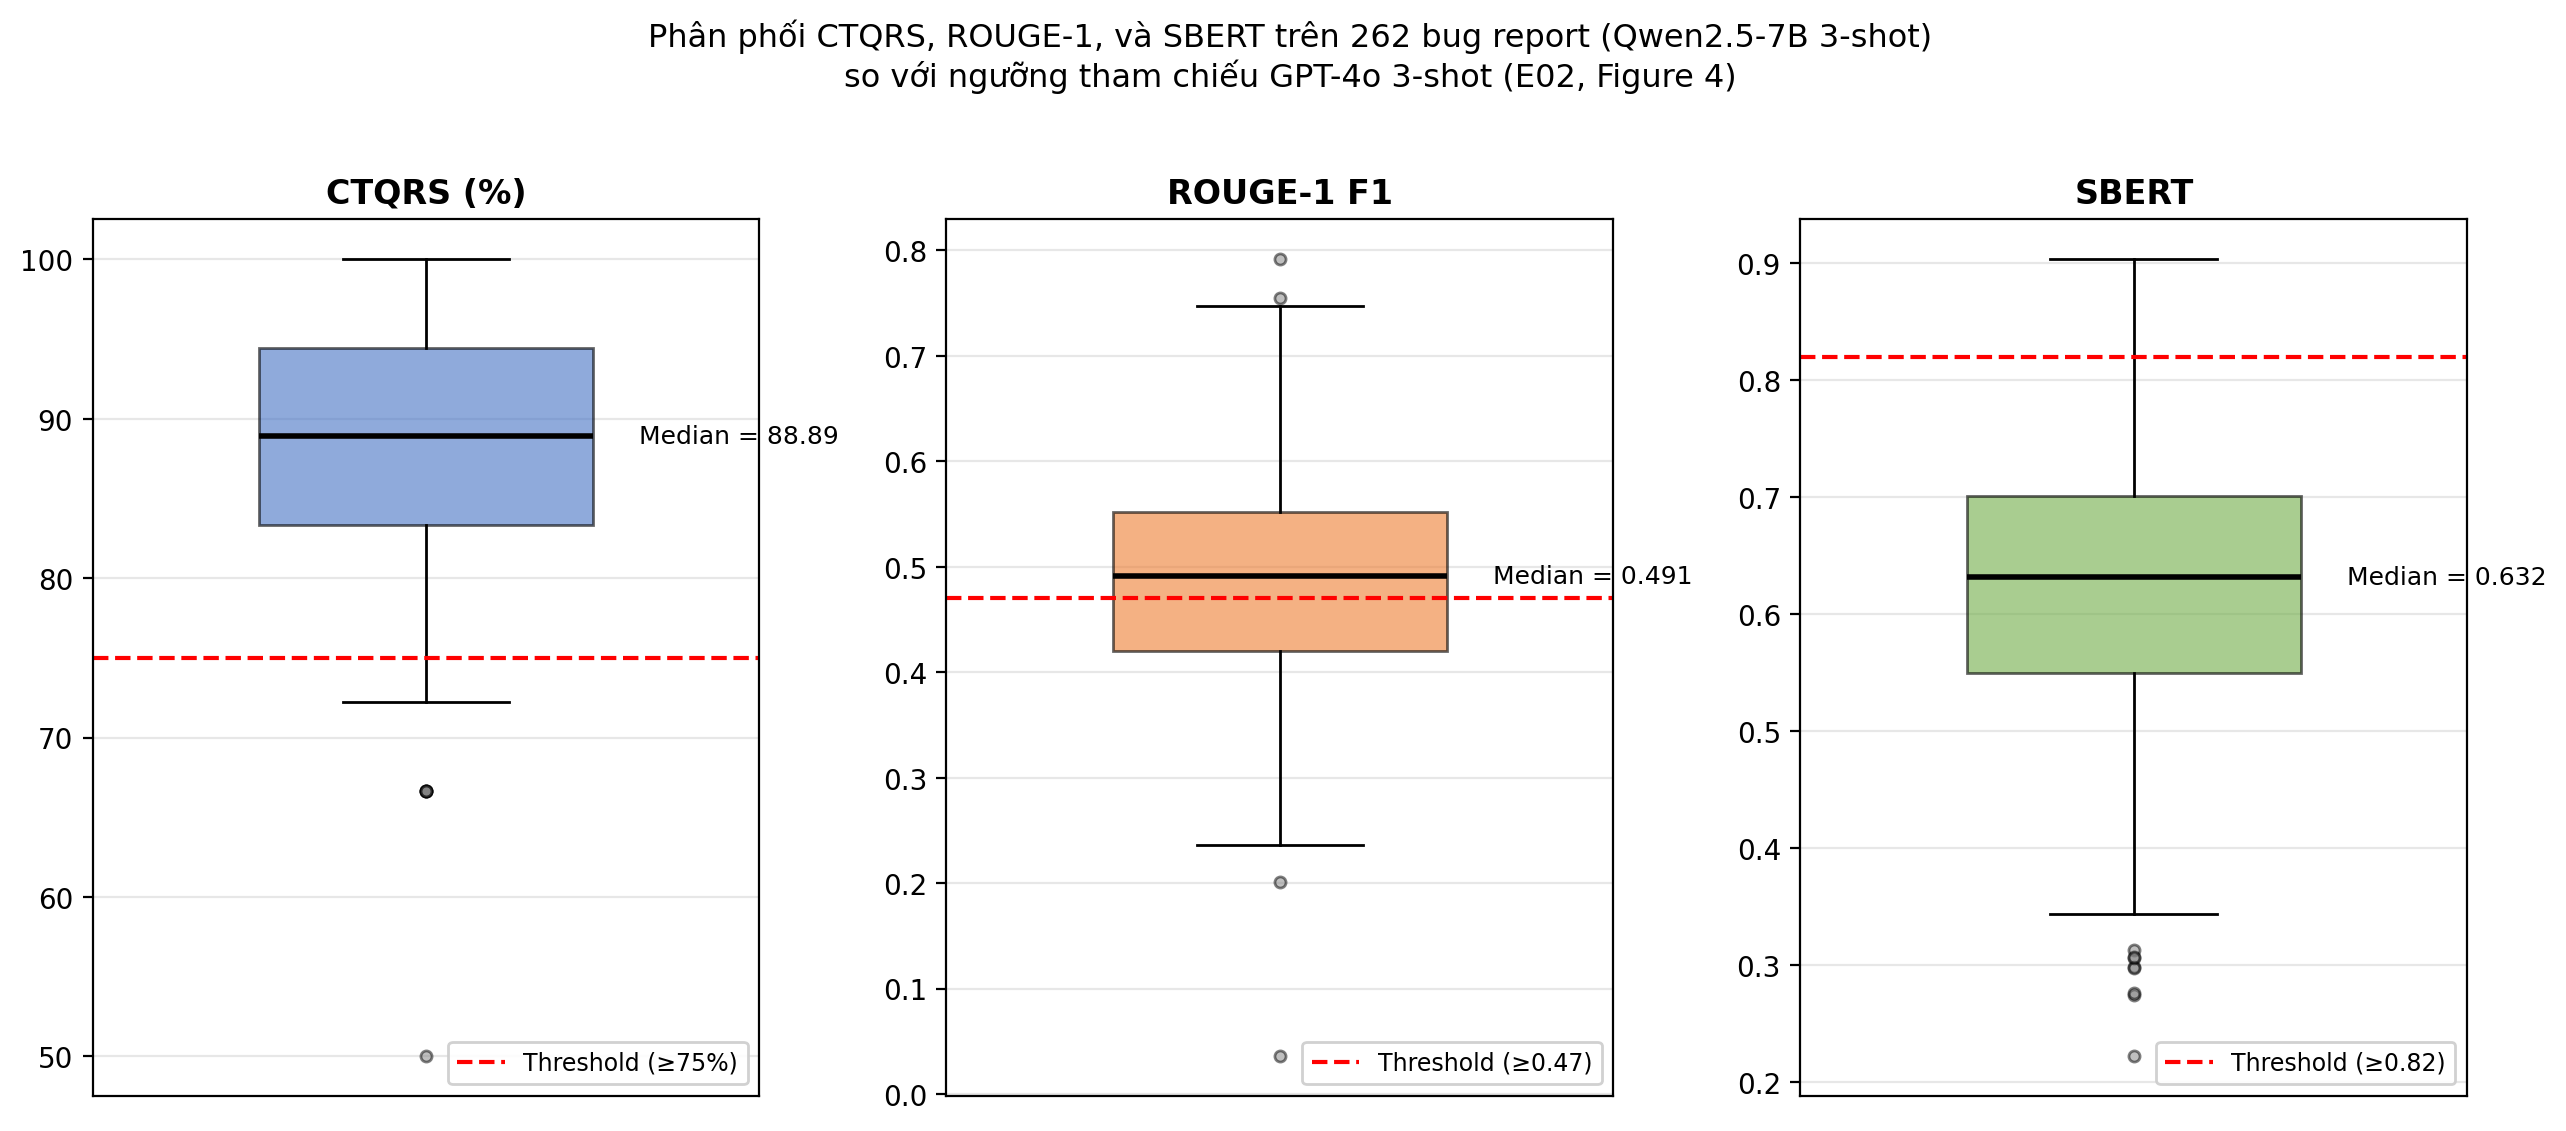
\includegraphics[width=\columnwidth]{figures/figure1_boxplot.png}
\caption{Distributions of CTQRS (\%), ROUGE-1 F1, and SBERT
scores obtained by Qwen2.5-7B with 3-shot prompting
(N=262). The dashed red lines represent the GPT-4o
reference thresholds reported by
\protect\cite{acharya2025bugquality}.}
\label{fig:boxplot}
\end{figure}

\textbf{Overall answer to RQ1.}

Across the three evaluation metrics, Qwen2.5-7B met the
published reference thresholds for CTQRS and ROUGE-1 F1.
However, the observed SBERT scores remained below the
corresponding GPT-4o reference threshold.

\section{Discussion}
\label{sec:discussion}

\subsection{Explaining the Main Findings}

\textbf{Why does CTQRS exceed the threshold by a large margin?}
Qwen2.5-7B 3-shot achieves median CTQRS=88.89\%, surpassing
the 75\% GPT-4o reference by 13.89 percentage points with a
large effect ($\delta=0.908$). CTQRS measures structural
completeness through rule-based sub-checks (presence of S2R,
EB, AB, environment information, interface elements). The
3-shot Alpaca-LoRA prompt explicitly instructs the model to
produce four sections, and Qwen reliably generates all required
structural components. This structural conformance is consistent
with E02's observation that even fine-tuned models achieve
high CTQRS scores once they learn the target
template~\cite{acharya2025bugquality}.

\textbf{Why does SBERT fall substantially below the threshold?}
Our length analysis reveals that Qwen outputs are on average
1.82$\times$ longer than the Bugzilla ground-truth reports
(245.5 words vs.\ 162.0 words). Qwen produces verbose,
markdown-formatted responses with section headers (e.g.,
\texttt{\#\#\#\# Steps to Reproduce}) and detailed bullet
points, whereas Bugzilla ground-truth reports are written in
plain, concise technical prose without headers. The
\texttt{paraphrase-MiniLM-L6-v2} encoder encodes the entire
passage into a fixed-size vector, making cosine similarity
sensitive to differences in length and formatting style
beyond semantic content. E02 itself notes that ``differences
in the length of the bug report generated can lead to unfair
comparisons in n-gram overlap
metrics''~\cite{acharya2025bugquality}; our results show
this effect extends to SBERT as well.

To confirm that the SBERT gap is caused by style rather than
semantic content, we conducted an ablation study adding a
length constraint to the system prompt (``keep total output
under 150 words''). While this shortened Qwen outputs to a
mean of 109.1 words (0.70$\times$ GT), SBERT further
decreased from 0.632 to 0.609. This counter-intuitive
result confirms that the problem is \emph{style mismatch},
not verbosity alone: outputs shorter than GT are penalized
in the opposite direction. ROUGE-1 improved from 0.491 to
0.532 with the length constraint, consistent with higher
unigram overlap when outputs are more concise.

\textbf{Why does ROUGE-1 achieve only a small effect?}
Median ROUGE-1=0.491 exceeds the 0.47 threshold but with a
small effect size ($\delta=0.191$). The margin above threshold
is narrow (0.021 F1 points), suggesting lexical overlap is
adequate but not strongly superior to the GPT-4o baseline.
This is consistent with E02's ROUGE results for fine-tuned
models on the S2R section (ROUGE=0.52), where the detailed
and lengthy S2R content also suppressed overlap
scores~\cite{acharya2025bugquality}.

\subsection{Comparison with Prior Work}

Our CTQRS result (88.89\%) substantially exceeds those
reported for fine-tuned models: Qwen2.5-7B fine-tuned
achieves 77\%~\cite{acharya2025bugquality}, AgentReport
with QLoRA achieves 80.5\%~\cite{choi2025agentreport},
and PPO reinforcement learning yields
76\%~\cite{yang2025ctqrsrl}. Three factors explain this:
(1) CTQRS measures structural completeness, which few-shot
prompting achieves readily when the prompt template
explicitly names all required sections; (2) our corrected
scorer (\texttt{max\_possible=18}) differs from the
original GindeLab scorer (\texttt{max\_possible=16}),
making direct numeric comparison with prior work
approximate; (3) fine-tuned models may produce shorter,
stylistically closer outputs that trade CTQRS for better
SBERT.

Our SBERT (0.632) is lower than the GPT-4o reference
(0.82) and likely lower than fine-tuned models, which
are trained to reproduce the exact style of Bugzilla
ground-truth reports. This confirms that few-shot
prompting, while effective for structural quality, cannot
replicate the writing style of domain-specific fine-tuned
models without additional training.

\subsection{Implications}

\textbf{For budget-constrained teams.}
Qwen2.5-7B 3-shot prompting --- requiring no GPU training,
no labeled data, and zero API cost when run on free cloud
compute --- produces structurally complete bug reports
(CTQRS=88.89\%) and adequate lexical fidelity
(ROUGE-1=0.491) that both exceed published GPT-4o few-shot
benchmarks. Teams lacking the resources to fine-tune a
model or subscribe to a proprietary API can adopt this
zero-training approach without sacrificing structural
quality. The only limitation is output verbosity, which
affects SBERT but not the structural completeness
perceived by developers reviewing the report.

\textbf{For researchers choosing evaluation metrics.}
SBERT similarity is sensitive to stylistic differences
between generated and reference texts beyond semantic
content. When the generation model and the reference corpus
have systematically different writing styles, SBERT scores
reflect style mismatch rather than content quality.
Researchers evaluating LLM-generated bug reports should
complement SBERT with style-agnostic metrics such as CTQRS
or human evaluation when the target style is not enforced
by the prompt.

\textbf{For practitioners choosing between few-shot and fine-tuning.}
Our findings support a practical decision rule: use
few-shot prompting when structural completeness (CTQRS) is
the primary requirement and compute budget is limited;
invest in fine-tuning when style alignment with a specific
reference corpus (SBERT) is required. Prior
work~\cite{acharya2025bugquality, choi2025agentreport,
yang2025ctqrsrl} shows that fine-tuned models achieve
higher SBERT by learning to replicate the exact writing
style of Bugzilla reports. The two approaches are
complementary: few-shot prompting provides a useful
starting point that fine-tuning can then refine for style.

\section{Threats to Validity}
\label{sec:threats}

We discuss threats to validity following the taxonomy of Wohlin et al.~\cite{wohlin2012experimentation}.

\subsection{Internal Validity}

\textbf{Model version drift.}
The \texttt{unsloth/Qwen2.5-7B-Instruct} checkpoint on HuggingFace
may be silently updated between setup and the full run, affecting
reproducibility. We mitigated this by pinning the exact model
revision at download time and logging all inference configuration
in \texttt{results/full\_api\_log.txt}.

\textbf{Non-zero temperature.}
Qwen2.5-7B-Instruct requires \texttt{temperature~>~0}; we used the
minimum permitted value of 0.01. To ensure deterministic decoding
we set \texttt{do\_sample=False} (greedy), which suppresses the
effect of temperature on output selection.

\textbf{Unspecified GPT-4o version in reference paper.}
E02~\cite{acharya2025bugquality} reports threshold values
(CTQRS=75\%, SBERT=0.82, ROUGE-1=0.47) attributed to
``ChatGPT-4o'' without specifying the exact model version string
(e.g., \texttt{gpt-4o-2024-08-06}). Notably, reference [53] within
E02 cites ``ChatGPT (Version 3.5)'' while Figure~4 reports
``ChatGPT 4o'', indicating an internal inconsistency in the source
paper. We therefore treat the published thresholds as historical
reference points rather than guaranteed reproducible values tied
to a fixed model version.

\subsection{External Validity}

\textbf{Single domain.}
Our test set is drawn exclusively from the Bugzilla/Mozilla domain.
Results may not generalize to other bug tracking systems or
application domains. We scoped our conclusions to the Bugzilla
domain and note cross-domain generalization as future work
(Section~\ref{sec:conclusion}).

\textbf{Limited cross-domain data.}
Our study does not include a cross-domain evaluation (originally
planned as RQ2 using 37 Mojira/Minecraft pairs from
E03~\cite{akyol2026improbr}). On closer inspection of the
full text of E03, those 37 pairs constitute a curated internal
set used for the ImproBR/ChatBR comparison and are not
available as a reusable public corpus. We therefore excluded RQ2
from the final scope and flag cross-domain validation as an open
research direction.

\subsection{Construct Validity}

\textbf{Non-overlapping test splits.}
Our test set (N=262) was produced by a 80/10/10 split with
\texttt{random\_state=42}; E02 used N=3,903 after an additional
SBERT-based deduplication step with an undisclosed seed,
yielding N=391 test samples. The two test sets are unlikely to be
identical, so published thresholds represent reference baselines
rather than results on the same data.

\textbf{Absence of paired baseline.}
We cannot perform paired significance testing between Qwen and
GPT-4o because per-instance GPT-4o outputs are not publicly
available. This limitation is acknowledged by prior
work~\cite{choi2025agentreport}, which states that
``paired significance testing not feasible due to unavailability
of per-instance baseline results.'' We adopt one-sample
Wilcoxon tests against the published threshold medians as
the methodologically sound alternative.

\textbf{CTQRS scorer discrepancy.}
The GindeLab scorer~\cite{acharya2025bugquality} hard-codes
\texttt{max\_possible=16}, while E02 reports a maximum of 17 in
the paper text. Computing the true maximum from the 13
sub-check weights in the scorer source code yields 18 (RM1--4:
$4\times1$; RR1/RR2/RR4/RR5: $4\times1$; RR3: $1\times2$;
RA1--4: $4\times2$). We used \texttt{max\_possible=18} as the
only value derivable from first principles without ambiguity,
ensuring CTQRS percentages remain bounded in $[0, 100]$.
We also corrected word-list noise in the RA sub-checks
(tokens shorter than 3 characters or containing whitespace
were removed) and applied whole-word boundary matching
to prevent spurious matches; details are in
\texttt{scripts/ctqrs\_scorer\_v2\_fixed.py}.

\textbf{Metric sensitivity to style.}
SBERT (\texttt{paraphrase-MiniLM-L6-v2}) encodes entire
passages into fixed-size vectors and is sensitive to differences
in length and formatting style, not only semantic content.
Our ablation (Section~\ref{sec:discussion}) confirms that
Qwen outputs are approximately 1.82$\times$ longer than
ground-truth reports and use markdown headers absent
from the plain-text Bugzilla reference reports, which
depresses cosine similarity independently of content quality.
CTQRS and ROUGE-1 provide complementary perspectives
that are less affected by this style gap.

\subsection{Conclusion Validity}

\textbf{Multiple testing.}
RQ1 involves three separate Wilcoxon tests (CTQRS, SBERT,
ROUGE-1), inflating the familywise Type~I error rate.
We applied Bonferroni correction ($\alpha_{\text{adj}} =
0.05/3 \approx 0.017$) and report both raw and
corrected $p$-values; the conclusions are unchanged
after correction.

\textbf{Effect size reporting.}
$p$-values alone do not quantify practical importance.
We therefore report Cliff's $\delta$ alongside every
Wilcoxon test~\cite{arcuri2011practical}, interpreted
using the conventional thresholds ($|\delta|<0.147$:
negligible; $<0.33$: small; $<0.474$: medium; otherwise
large).

% sections/07_conclusion.tex
% §7 Conclusion — RW (Võ Thanh Phong, SE194101)
% Nguồn: RQ1_results_FINAL.md + full_metrics_output_FINAL.csv + proposal.md §4

\section{Conclusion}
\label{sec:conclusion}

We investigated whether Qwen2.5-7B-Instruct with 3-shot prompting
can match the quality thresholds established by GPT-4o 3-shot
(CTQRS$\geq$75\%, SBERT$\geq$0.82, ROUGE-1$\geq$0.47)
on 262 Bugzilla bug reports~\cite{acharya2025bugquality}.
Our results are mixed. Qwen2.5-7B few-shot exceeds the
structural quality threshold (median CTQRS=88.89\%,
$p<0.001$, $\delta=0.908$, large) and the lexical overlap
threshold (median ROUGE-1=0.491, $p=0.002$, $\delta=0.191$,
small), but falls substantially below the semantic
similarity threshold (median SBERT=0.632, $p=1.000$,
$\delta=-0.969$, large). An ablation study adding a
length constraint to the prompt improved ROUGE-1
(0.491$\rightarrow$0.532) but further reduced SBERT
(0.632$\rightarrow$0.609), confirming that the SBERT
deficit stems from output style mismatch rather than
semantic content errors.

This is the first study to directly evaluate Qwen2.5-7B
few-shot prompting against published GPT-4o few-shot thresholds
on the bug report restructuring task. Our findings suggest
that, for organizations with limited GPU resources that
cannot afford fine-tuning, Qwen2.5-7B 3-shot prompting is
a viable option for producing structurally complete bug reports
(CTQRS) with adequate lexical fidelity (ROUGE-1), but style
alignment with Bugzilla-style ground-truth reports remains
an open challenge that few-shot prompting alone cannot resolve.

Future work could investigate three concrete directions:
(1) applying style-specific constraints or in-context style
exemplars that more precisely match the plain-text, concise
Bugzilla writing style to close the SBERT gap without
fine-tuning;
(2) cross-domain evaluation on Mojira/Minecraft or mobile
app bug trackers to assess generalizability beyond Mozilla
projects;
(3) lightweight parameter-efficient fine-tuning (e.g.,
LoRA~\cite{acharya2025bugquality}) on a small domain-specific
sample to quantify the minimum training investment needed
to close the remaining gap.

Our replication package --- including the dataset split,
3-shot prompt template, inference scripts, metric scorer,
and raw results --- is publicly available at
\url{https://github.com/HoangThong05/RT-SWT-003-nhom3}.

\bibliographystyle{IEEEtran}
\bibliography{references}
\end{document}